\documentclass[11pt,a4paper]{article}
\usepackage[utf8]{inputenc}
\usepackage[T1]{fontenc}
\usepackage[spanish]{babel}
\usepackage[margin=2.2cm]{geometry}
\usepackage{tabularx}
\usepackage{booktabs}
\usepackage{graphicx}
\usepackage{float}

\setlength{\parindent}{0pt}
\setlength{\parskip}{0.5em}

\begin{document}

\begin{center}
    \textbf{\Large Universidad Técnica Estatal de Quevedo}\\
    \textbf{Facultad de Ciencias de la Computación -- Carrera de Software}\\
    \textbf{Ingeniería de Requerimientos (ISR-401) -- Evaluación EV-PRAC-01}
\end{center}

\vspace{0.3cm}
\textit{Esta es la transcripción fiel de la prueba escrita a mano el 18/11/2026; las fotografías de las hojas están en el anexo.}
\vspace{0.3cm}

\hrule
\vspace{0.3cm}

\textbf{Apellidos y Nombres:} Chalacan Yerovi David \\
\textbf{Fecha:} 18/11/2026

\section*{T1}

\textbf{T1(a):} un requisito es una condicion expuesta en un sistema que se debe cumplir para que el sitema satisfaga / resuelva el problema concordado.

E7, No es un requisito porque solo describe la situación actual del proceso manual

E12, No es un requisito del producto, debido a que es mas bien un requisito del proceso

\textbf{(b):} StRS: Especifica las necesidades, expectativas y restricciones de los interesados

E1, <<Necesitamos enterarnos de inmediato cuando una refrigeradora se salga de rango, aunque sea de madrugada>>, una necesidad operativa de la coordinadora de inmunizaciones

SyRS: Habla sobre los requisitos de manera global

E3, define una restriccion de interfaz del hardware y el protocolo

SRS : Capacidades funcionales y que el software especifico debe implementar

E5, describe una capacidad automatizada directa del software

\textbf{(c):} H1: Actividad de Elicitación. En el marco de Phol es una actividad central

H2: Actividad de analisis y negociación. En el marco de Pohl es una actividad central

H3: Actividad de Especificacion. En el marco de Pohl es una actividad central

H4: Actividad de Validacion. En el maro de Pohl es una actividad central

H5: Actividad de Gestion de requisitos. En el marco de Pohl es una actividad transversal

\section*{T2 (a):}

\begin{table}[H]
\centering
\renewcommand{\arraystretch}{1.35}
\begin{tabularx}{\textwidth}{|l|l|l|X|}
\hline
\textbf{ID} & \textbf{Tipo} & \textbf{Documento} & \textbf{Justificación} \\ \hline
E1 & Funcional & SRS & Capacidad del software para notificar alertas de exursion termica \\ \hline
E2 & Requisito de dominio & SyRS/SRS & Regla de negocio de salud publica \\ \hline
E3 & Restriccion (Hardware/Protocolo) & SyRS & Condicion externa impuesta por el uso obligatorio del sensor \\ \hline
E4 & Restricción (Plazo y Presupuesto) & StRS & Limite temporal y economico fijado por la directiva \\ \hline
E5 & Funcional & SRS & Capacidad del software para generar informes mensuales \\ \hline
E6 & No funcionla & SyRS & Capacidad de operar y registrar durante cortes electricos \\ \hline
E7 & No es un requisito & Ninguno & Describe el procedimiento manual actual, no el sistema a construir \\ \hline
E8 & No funcional & SRS & Tiempo de respuesta del sistema \\ \hline
E9 & Restricción & SyRS & Obligacion tecnica de instalar la plataforma en el servidor Linux \\ \hline
E10 & Funcional / Seguridad & SRS & Control de permisos de usuarios y trazabilidad de acciones correctivas \\ \hline
E11 & No funcional & SRS & Tiempo de aprendizaje o facilidad de uso para un usuario novato \\ \hline
E12 & Requisito de proceso / gestion & Ninguno & Regla la organización de actividades y firmas del proyecto de desarrollo \\ \hline
\end{tabularx}
\end{table}

\section*{b):}

\begin{table}[H]
\centering
\renewcommand{\arraystretch}{1.35}
\begin{tabularx}{\textwidth}{|l|X|X|X|}
\hline
\textbf{ID} & \textbf{Termino} & \textbf{Caracteristica 29148} & \textbf{Propiedad SMART} \\ \hline
B1 & ``rapido y facil de usar'' & No ambigua / verificable & Medible / Especifico \\ \hline
B2 & ``oportuna'' ``temperatura inadecuada'' & No ambigua / Completa & Especifico / Medible \\ \hline
B3 & ``En todo momento, incluso sin energia'' & Realizable / Factible & Attainable / Realizable \\ \hline
B4 & ``Mongo DB alojada en la nube AWS'' & Consistente & Attainable \\ \hline
B5 & ``Si es posible'' ``etc'' & Completa / verificable & Especifico / Medible \\ \hline
B6 & Ninguno & Cumple la clausula 5.2.4 & Cumple con todas las propiedades Smart \\ \hline
\end{tabularx}
\end{table}

\newpage
\section*{Anexo: Evidencias fotográficas de las hojas originales}

\begin{figure}[H]
    \centering
    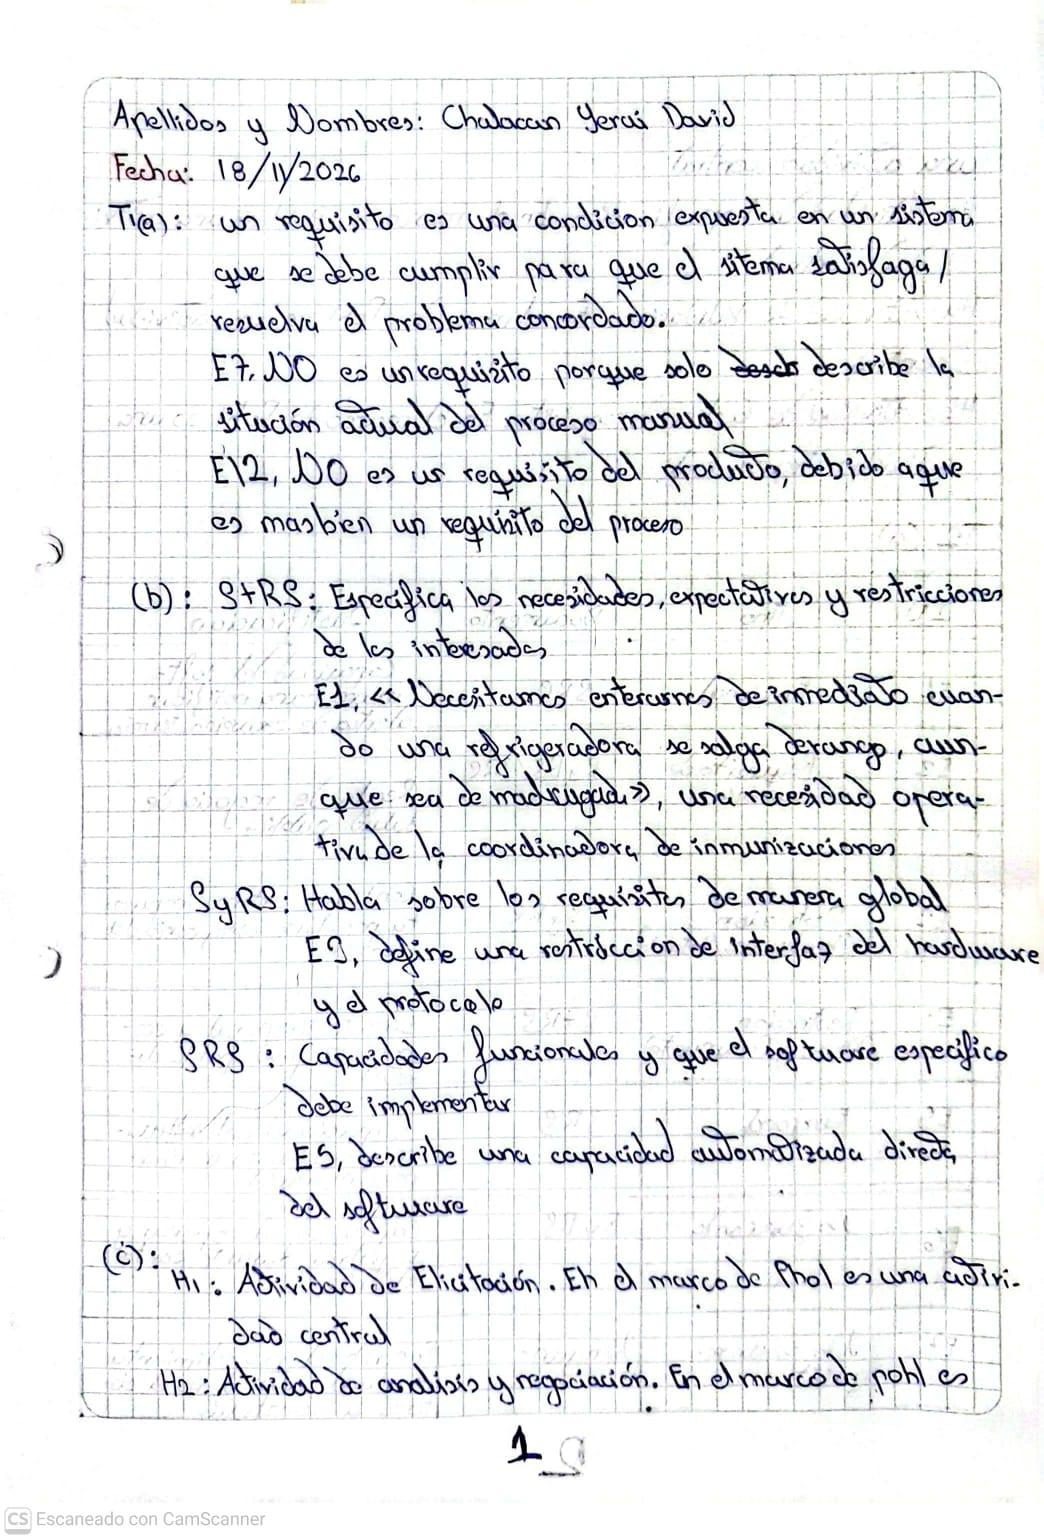
\includegraphics[width=0.88\textwidth]{evidencias/hoja-01.jpeg}
    \caption{Hoja 1 de 3 de la evaluación escrita a mano.}
\end{figure}

\newpage
\begin{figure}[H]
    \centering
    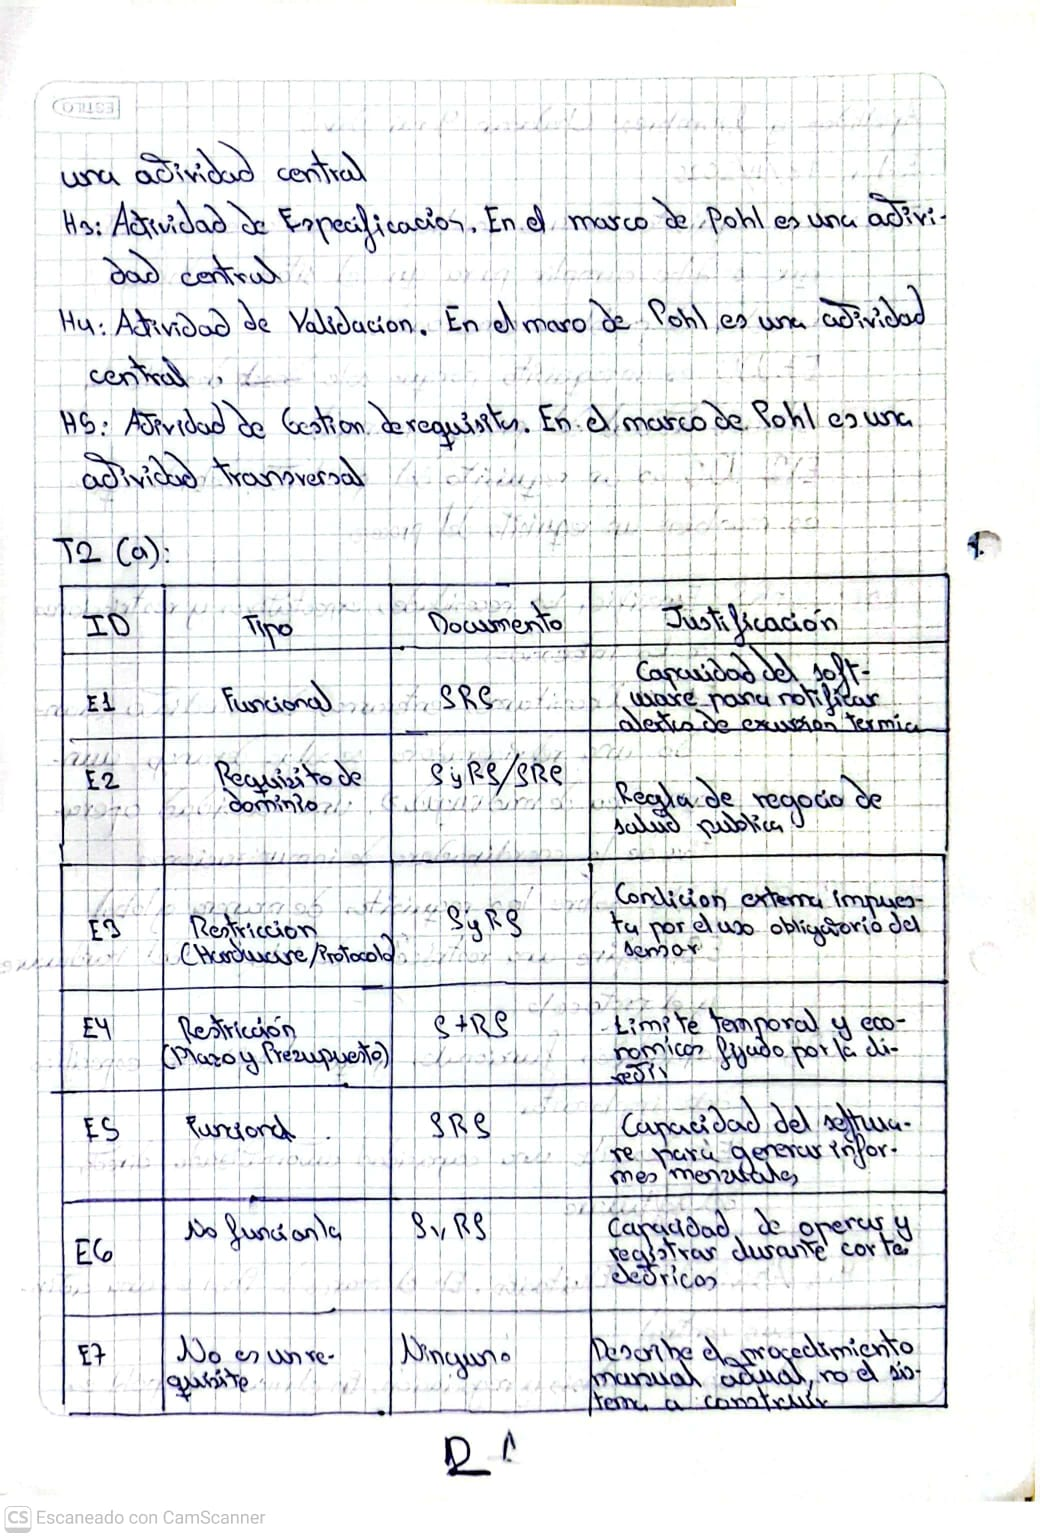
\includegraphics[width=0.88\textwidth]{evidencias/hoja-02.jpeg}
    \caption{Hoja 2 de 3 de la evaluación escrita a mano.}
\end{figure}

\newpage
\begin{figure}[H]
    \centering
    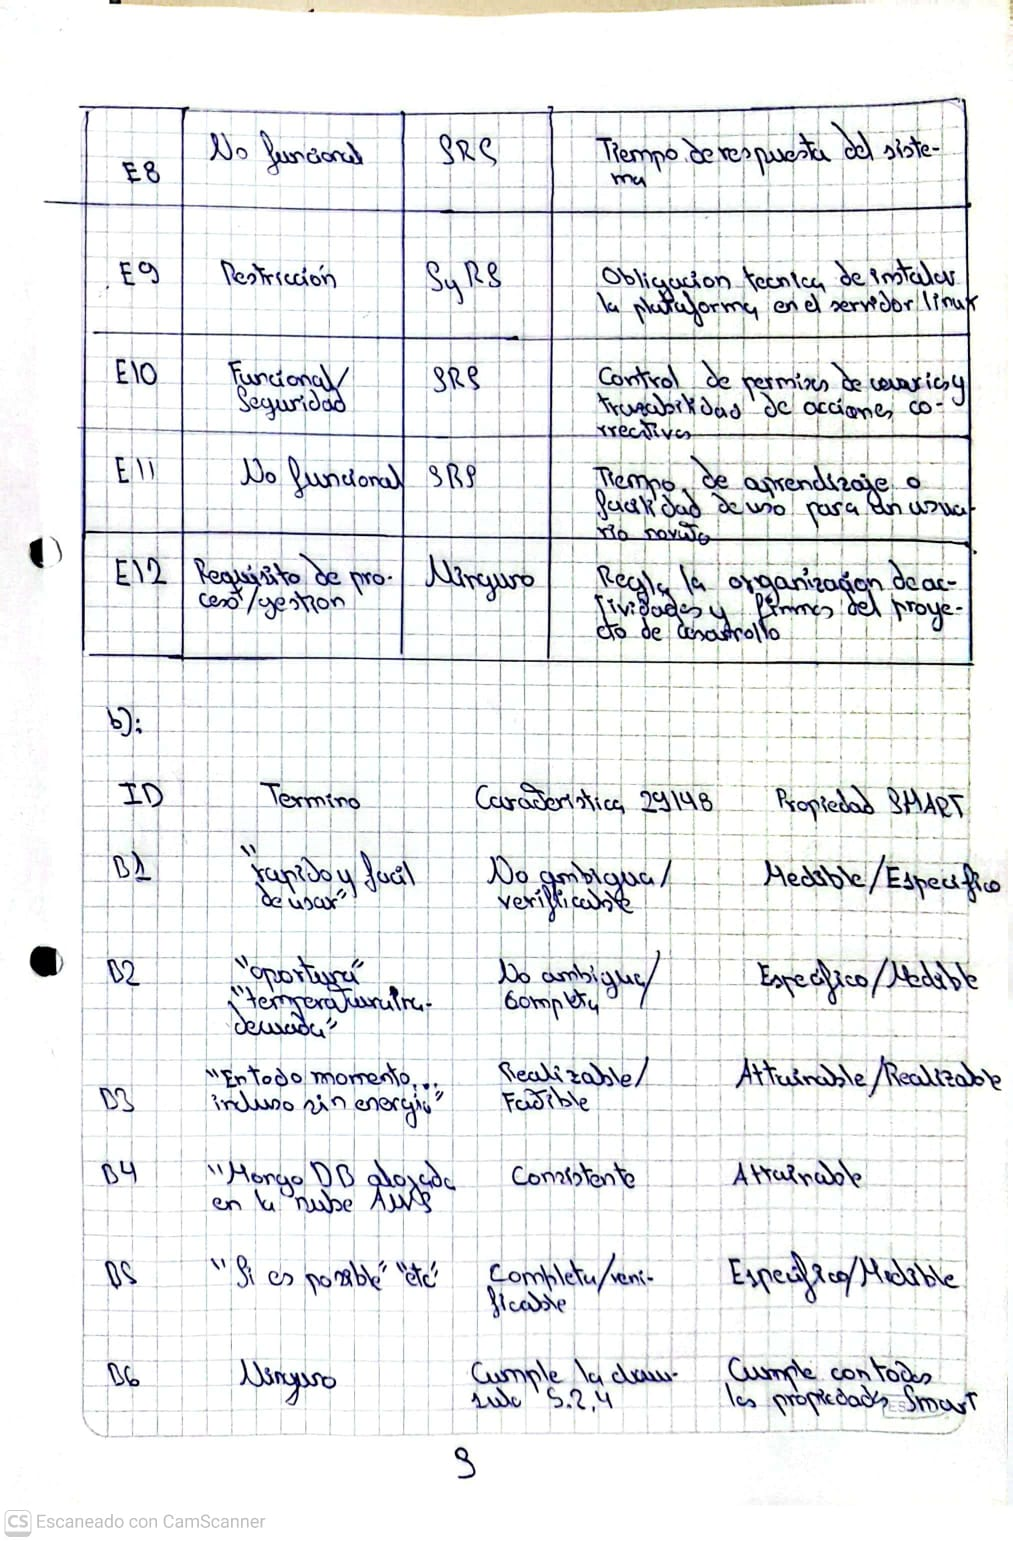
\includegraphics[width=0.88\textwidth]{evidencias/hoja-03.jpeg}
    \caption{Hoja 3 de 3 de la evaluación escrita a mano.}
\end{figure}

\end{document}
